% Source: graduate-coursework/Sp26/CSCE775/course_notes/practice_problems.tex

\documentclass[border=4pt]{standalone}
\usepackage{amsmath, amssymb, amsthm}
\usepackage{tikz}
\usepackage{xcolor}
\usetikzlibrary{arrows.meta, positioning, shapes.geometric}

\definecolor{Garnet}{RGB}{115, 0, 10}
\definecolor{Atlantic}{RGB}{70, 106, 159}
\definecolor{Congaree}{RGB}{31, 65, 77}
\definecolor{NinetyBlack}{RGB}{54, 54, 54}
\definecolor{FiftyBlack}{RGB}{162, 162, 162}

\begin{document}
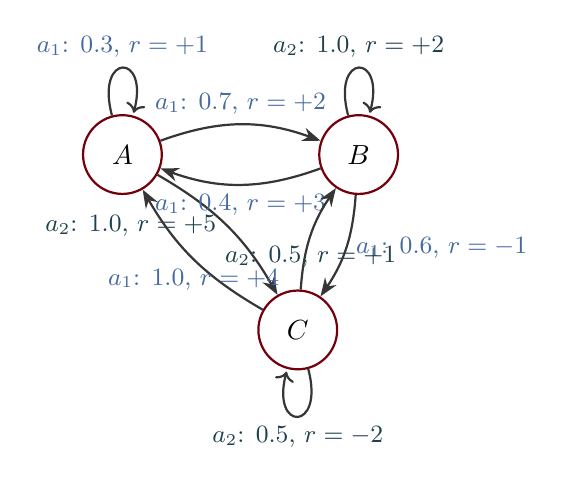
\begin{tikzpicture}[
    node distance=3cm,
    state/.style={circle, draw=Garnet, thick, minimum size=1cm},
    action/.style={font=\small},
    every edge/.style={draw=NinetyBlack, thick, -Stealth}
]

% States
\node[state] (A) {$A$};
\node[state, right of=A] (B) {$B$};
\node[state, below right=1.5cm and 1.5cm of A] (C) {$C$};

% From A
\draw[Atlantic] (A) edge[bend left=20] node[above, action] {$a_1$: 0.7, $r=+2$} (B);
\draw[Atlantic] (A) edge[loop above] node[above, action] {$a_1$: 0.3, $r=+1$} (A);
\draw[Congaree] (A) edge[bend left=15] node[left, action] {$a_2$: 1.0, $r=+5$} (C);

% From B
\draw[Atlantic] (B) edge[bend left=20] node[below, action] {$a_1$: 0.4, $r=+3$} (A);
\draw[Atlantic] (B) edge[bend left=15] node[right, action] {$a_1$: 0.6, $r=-1$} (C);
\draw[Congaree] (B) edge[loop above] node[above, action] {$a_2$: 1.0, $r=+2$} (B);

% From C
\draw[Atlantic] (C) edge[bend left=15] node[below, action] {$a_1$: 1.0, $r=+4$} (A);
\draw[Congaree] (C) edge[bend left=15] node[below, action] {$a_2$: 0.5, $r=+1$} (B);
\draw[Congaree] (C) edge[loop below] node[below, action] {$a_2$: 0.5, $r=-2$} (C);

\end{tikzpicture}
\end{document}
